\let\negmedspace\undefined
\let\negthickspace\undefined
\documentclass[journal]{IEEEtran}
\usepackage[a5paper, margin=10mm, onecolumn]{geometry}
%\usepackage{lmodern} % Ensure lmodern is loaded for pdflatex
\usepackage{tfrupee} % Include tfrupee package

\setlength{\headheight}{1cm} % Set the height of the header box
\setlength{\headsep}{0mm}     % Set the distance between the header box and the top of the text

\usepackage{gvv-book}
\usepackage{gvv}
\usepackage{cite}
\usepackage{amsmath,amssymb,amsfonts,amsthm}
\usepackage{algorithmic}
\usepackage{graphicx}
\usepackage{textcomp}
\usepackage{xcolor}
\usepackage{txfonts}
\usepackage{listings}
\usepackage{enumitem}
\usepackage{mathtools}
\usepackage{gensymb}
\usepackage{comment}
\usepackage[breaklinks=true]{hyperref}
\usepackage{tkz-euclide} 
\usepackage{listings}
% \usepackage{gvv}                                        
\def\inputGnumericTable{}                                 
\usepackage[latin1]{inputenc}                                
\usepackage{color}                                            
\usepackage{array}                                            
\usepackage{longtable}                                       
\usepackage{calc}                                             
\usepackage{multirow}                                         
\usepackage{hhline}                                           
\usepackage{ifthen}                                           
\usepackage{lscape}
\usepackage{xr}
\externaldocument{/home/homa/Desktop/matgeo/main}
\begin{document}

\bibliographystyle{IEEEtran}
\vspace{3cm}

\title{1-1.9-21}
\author{EE24BTECH11062 - Homa Harshitha Vuddanti
}
% \maketitle
% \newpage
% \bigskip
{\let\newpage\relax\maketitle}

\renewcommand{\thefigure}{\theenumi}
\renewcommand{\thetable}{\theenumi}
\setlength{\intextsep}{10pt} % Space between text and floats


\numberwithin{equation}{enumi}
\numberwithin{figure}{enumi}
\renewcommand{\thetable}{\theenumi}


\textbf{Question}:\\
Given vertices of a parallelogram $\vec{A}=\myvec{-2\\1}, \vec{B}=\myvec{a\\0}, \vec{C}=\myvec{4\\b},$ and $\vec{D}=\myvec{1\\2}$. Find the values of $a$ and $b$. Hence, find the lengths of its sides.
\\
\textbf{Solution: }\\
\begin{table}[h!]    
  \centering
  \begin{tabular}[12pt]{ |c| c|}
    \hline
    \textbf{Variable} & \textbf{Description}\\ 
    \hline
    $a$ & $x$-coordinate of point B\\
    \hline 
    $b$ & $y$-coordinate of point C\\
    \hline
    \end{tabular}


  \caption{Variables Used}
  \label{1-1.9-21-table}
\end{table}
Given, the sides of the parallelogram.\\In a parallelogram $ABCD$, 
since $AB$ is parallel to $CD$,

From \eqref{eq:two-pgm},
\begin{align}
    \vec{B}-\vec{A}=\vec{C}-\vec{D}
\end{align}

 \begin{align}
\myvec{a-(-2)\\0-1}&=\myvec{4-1\\b-2}\label{1-1.9-21-1}\\
\myvec{a+2\\-1}&=\myvec{3\\b-2}\label{1-1.9-21-2}\\
a+2&=3\label{1-1.9-21-3}\\
b-2&=-1\label{1-1.9-21-4}
\end{align}
 From equations \eqref{1-1.9-21-3} and \eqref{1-1.9-21-4}, 
\begin{align}
a&=1,\\
b&=1
\end{align}
To find lengths of sides,
\begin{align}
AB=CD&=\sqrt{\brak{A-B}^\top\brak{A-B}}\\
&=\sqrt{A^\top A-A^\top B -B^\top A+B^\top B }\label{1-1.9-21-5}\\
AD=BC&=\sqrt{\brak{A-D}^\top\brak{A-D}}\\
&=\sqrt{A^\top A-A^\top D -D^\top A+D^\top D }\label{1-1.9-21-6}\\
\end{align}
Substituting values,
\begin{align}
AB&=\sqrt{\myvec{-3\\1}^\top \myvec{-3\\1}}=\sqrt{\brak{-3}\brak{-3}+\brak{1}\brak{1}}\\
AB=CD&=\sqrt{10}\label{1-1.9-21-7}\\
AD&=\sqrt{\myvec{-3\\-1}^\top \myvec{-3\\-1}}=\sqrt{\brak{-3}\brak{-3}+\brak{-1}\brak{-1}}\\
AD=BC&=\sqrt{10}\label{1-1.9-21-8}
\end{align}
\begin{figure}[h!]
   \centering
   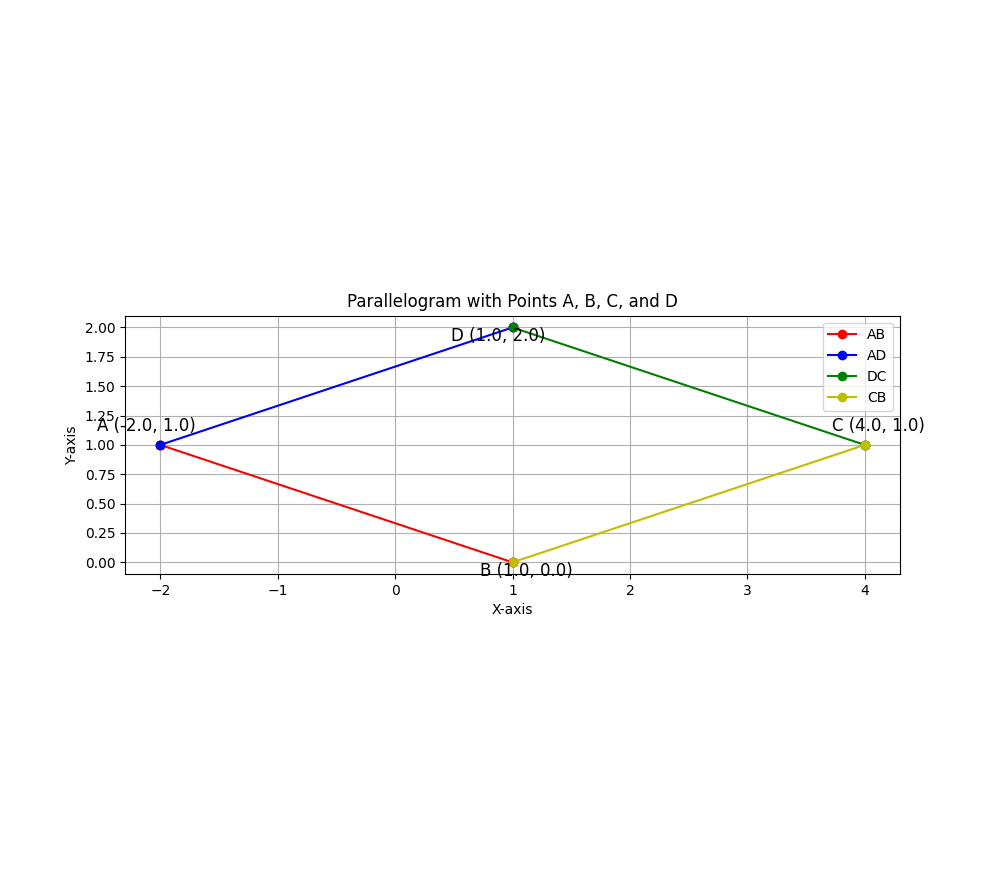
\includegraphics[width=1.1\columnwidth]{Figs/Figure_1.png}
   \caption{Plot}
   \label{1-1.9-21-fig-1}
\end{figure}
\end{document}  




